
\subsection{Background}

Over the last few years, load growth, increases in intermittent generation,
declining technology costs and increasing recognition of the importance of
customer behaviour in energy markets have brought about a change in the
focus of DR in Europe [Tor10]. The long standing programmes involving large
industries, through interruptible tariffs and time of day pricing, have been
increasingly complemented by programmes aimed at commercial and residential
customer groups.

\cite{torriti_demand_2010} Tor10] examines experiences within European countries as well as at
European Union (EU) level. While business programmes, technical and economic
potentials vary across Europe, there are common reasons as to why
coordinated DR policies have been slow to emerge: the limited knowledge on
DR energy saving capacities; high cost estimates for DR technologies and
infrastructures; and policies focused on creating the conditions for
liberalising the EU energy markets.


advances in DR It describes initiatives, studies and policies of various
European countries, with in-depth case studies of the UK, Italy and Spain.

Spees, K., {\&} Lave, L. B. (2007). Demand Response and Electricity Market
Efficiency. \textit{The Electricity Journal}, \textit{20}(3), 69--85. doi:10.1016/j.tej.2007.01.006

Interruptible Programmes represent 6.5{\%} of peak power and Load Shedding
Programmes initiate automatic load shedding in emergency situations [30].
With Interruptible Programmes participants are required to reduce their load
to predefined values. With Load Shedding Programmes utilities have the
possibility to remotely shutdown participants' equipment at short notice.
One significant difference between these two programmes is that for
Interruptible Programmes participants who do not respond can face penalties.


Load Shedding Programmes are divided into real time programmes (without
notice) and 15 min notice programmes. The size ranges from 1200 MW for real
time programmes to 1750 MW for notice programmes. Participants in these
programmes have to install and maintain Load Shedding Peripheral Units and
will be compensated according to a non-market price defined in regulation.
The size of curtailable power is of 10 MW for programmes without notice and
3 MW for programmes with notice.

Load forecasting is very important for power system operation and planning.
Traditional load forecasting tools have limitations to reflect DR customer
behaviors into load predictions. In [Zhou12], existing DR contracts are
reviewed for both wholesale and retail markets. In this study, an
illustrative example is provided to explore the impact of these contracts on
load forecasting. In conclusion, a concept of proactive load forecasting
based on contract types is proposed for forecasting loads in a smart grid
environment.

Modern hardware components such as processor, memory, disk and network offer
feature sets (Burd and Brodersen, 1995) to support energy aware operations.
Exploiting these feature sets in order to be more energy efficient is a very
important and challenging task in modeling cost/performance trade-offs, in
designing algorithms, and in defining policies. Today processors offer two
power-aware features, i.e., cpuidle and Dynamic Voltage and Frequency
Scaling (DVFS). The cpuidle feature offers a number of CPU power states
(C-states) in which they could reduce power when CPU is idle by closing some
internal gates. The CPU C-states are C0, C1, ..., Cn. C0 is the normal
working state where CPU will execute instruction, and C1, ...,Cn are
sleeping state where CPU stops executing instruction and power down some
internal components to save power. The DVFS is another power-saving method
especially when CPUs are in load line, allowing quick adjustment to
frequency/voltage upon demand in small interval. The key idea behind DVFS
techniques is to dynamically scale the supply voltage level of the CPU so as
to provide just-enough circuit speed to process the system workload, thereby
reducing the energy consumption.

We received eleven responses from the following sites: LLNL, ANL, Intel,
SDSC, Illinois, NOAA, ORNL, Purdue, AF, NERSC, LANL. The table below shows
the ranks of the responding organization in the top 100 list. 80{\%} of the
top 10, 60{\%} of the top 50, and 30{\%} of the top 100 participated in the
survey.


\begin{table}[htbp]
\begin{center}
\caption{Participating organizations and their rank in the top 100.}
\begin{tabular}{|p{59pt}|l|l|l|l|l|l|l|l|l|l|l|}
\hline
Organization&
ORNL&
LLNL&
ANL&
LANL&
NERSC&
Purdue&
AF&
NOAA&
Intel&
SDSC&
Illinois \\
\hline
Rank&
2&
3&
5&
22&
24&
28&
40&
48&
71&
102&
 \\
\hline
\end{tabular}
\label{tab4}
\end{center}
\end{table}

The survey had a total of 29 questions, eight of the questions were skipped
16 times by the 11 participants. This is only 5{\%} of the total questions
answered by the eleven participants. The graph below shows the distribution
of skipped questions.


\begin{figure}
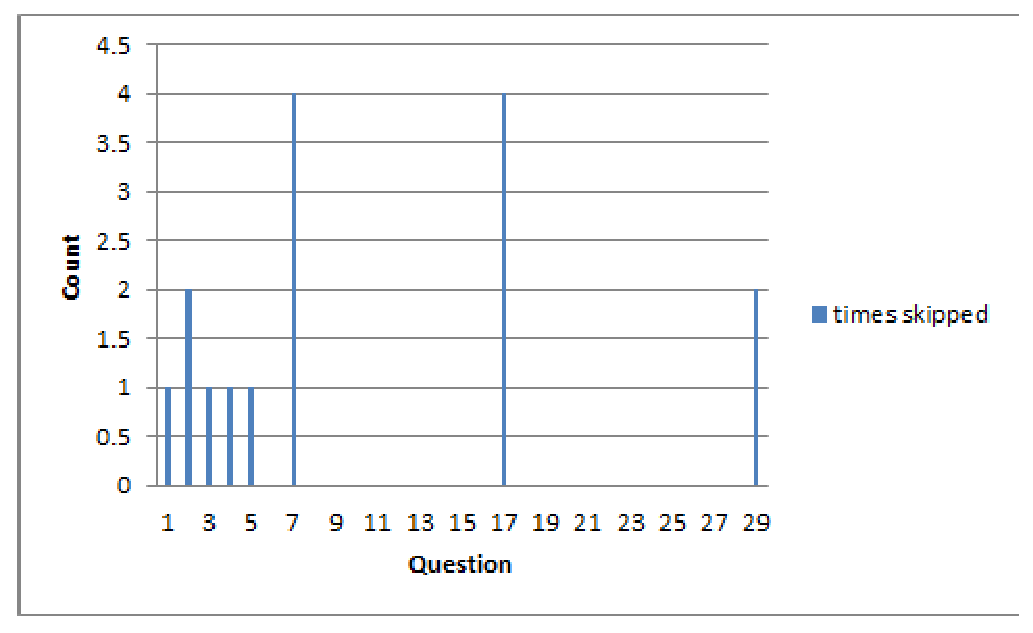
\includegraphics[width=4.01in,height=2.01in]{figure2}
\caption{Figure 2}
\end{figure}


Question 7 and 17 were skipped 4 times each, these two questions are follow
up questions to questions 6 and 16 and we were trying to collect more
details about user's responses in questions 6 and 16.
